\chapter{PCStream} 
\label{chap:PCstream}

\section{Introduction}
\label{sec:intro}
Multi-streamed SSDs provide a special mechanism,
called streams, for a host system to prevent data with different lifetimes 
from being mixed into the same block~\cite{T10, MultiStream}.
When the host system maps two data $D_1$ and $D_2$ to 
different streams $S_1$ and $S_2$, a multi-streamed SSD guarantees that 
$D_1$ and $D_2$ are placed in different blocks.   
Since streams, when properly managed, can be very effective in minimizing 
the copy cost of garbage collection (GC), they
can significantly improve both the performance and lifetime of 
flash-based SSDs~\cite{MultiStream, Level, FStream, AutoStream}.

In order to achieve high performance on multi-streamed SSDs, data with similar 
{\it future} update times~\cite{PCHa}
should be allocated 
to the same stream, so that the copy cost of GC can be minimized.
However, since it is difficult to know the future update times {\it a priori} when they are written,
stream allocation decisions are often {\it manually} made 
by programmers based on their expertise
on the application~\cite{MultiStream, Level} or the file system~\cite{FStream}.  
%Furthermore, these manual techniques assume 
%that the number of streams in an SSD is not changing, 
%thus requiring manual modifications whenever the number of streams in the SSD changes.
In this paper, our goal is to develop 
%a {\it fully automatic} technique for managing streams which is applicable for {\it any} multi-streamed SSD.
a {\it fully automatic} stream management technique. %which is applicable for multi-streamed SSD. %shane part

\subsection{Fallacy: LBA-based lifetime prediction}
Many existing data separation techniques such as~\cite{AutoStream, HotCold} 
estimate the data lifetime based on the update frequency of LBAs.  
For example, \textsf{\small AutoStream}~\cite{AutoStream} assumes that, if
some LBAs are frequently rewritten by applications, those LBAs hold hot data.
This LBA-based lifetime prediction 
approach, however, does not work well with recent data-intensive 
applications where a majority of
new data are written in an append-only manner.  



In order to illustrate a mismatch between an LBA-based predictor and 
append-only workloads, we analyzed the write pattern of 
RocksDB~\cite{RocksDB}, which is a
popular key-value store based on the LSM-tree algorithm~\cite{LSM}.
Fig.~\ref{fig:lba_lifetime}(a) shows how LBAs may be related 
to data lifetimes\footnote{The lifetime of data is defined 
by the logical time which is the number of writes to the device 
between when the data is first written 
and when the data is invalidated by an overwrite or a TRIM command.}
in RocksDB~\cite{RocksDB}.  
As shown in Fig.~\ref{fig:lba_lifetime}(a), 
there exists no strong correlation between the LBAs and lifetimes in RocksDB.  
This scatter plot is in sharp contrast with one for update workloads 
where a few distinct LBA regions have short lifetimes while others 
have very long lifetimes.

\begin{figure}[t]
	\centering
	\hfill
	%\subfigure[Lifetime patterns over LBAs]{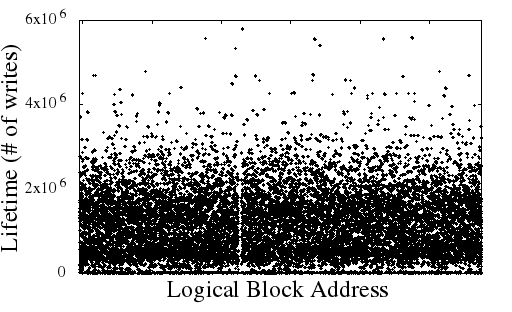
\includegraphics[width=0.215\textwidth]{figure/pcstream/lba_lifetime2}}  % data from 0/03031641
	\subfigure[Lifetime patterns over LBAs]{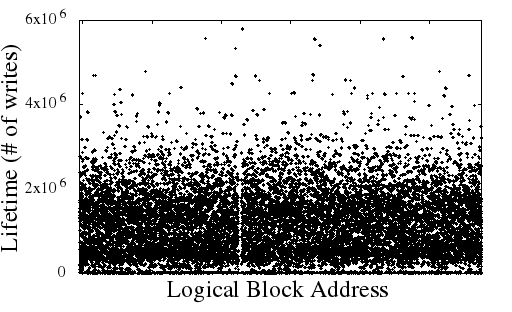
\includegraphics[scale=0.34]{figure/pcstream/lba_lifetime2}} \hspace{30pt}  % data from 0/03031641 
	\subfigure[Lifetime patterns over time]{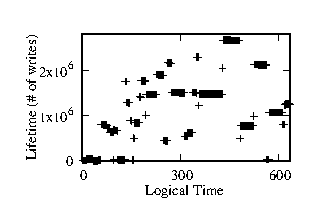
\includegraphics[scale=1]{figure/pcstream/lifetime_in_chunk}}
	%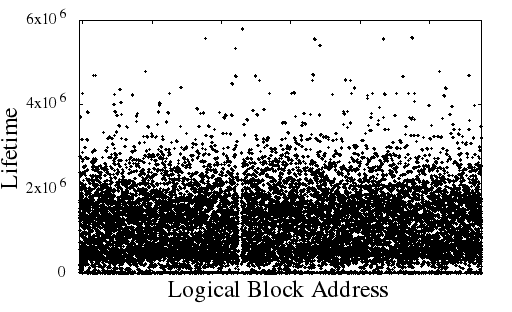
\includegraphics[width=0.9\linewidth]{figure/pcstream/lba_lifetime} 
	\caption{Lifetime distributions over addresses and times.} %shane part
	\label{fig:lba_lifetime}
\end{figure}


We also analyzed 
if the lifetimes of LBAs change under some predictable patterns over time 
although the overall lifetime distribution shows large variances.
Fig.~\ref{fig:lba_lifetime}(b) shows a scatter plot of data lifetimes over the logical time 
for a specific 1-MB chunk with 256 pages. 
As shown in Fig.~\ref{fig:lba_lifetime}(b), 
for the given chuck, data lifetimes vary in a random fashion
(although some temporal locality is observed).
\begin{comment}
Over the logical time, the lifetime of data written to the chunk 
varies in an unpredictable fashion.  
For example, at the logical time 10, the lifetime was 1 but it increases about 
2.6 million around the logical time 450 
followed by a rapid drop around the logical time 600. 
\end{comment}
Our illustration using RocksDB strongly suggests that under append-only
workloads, LBAs are not useful in deciding data lifetimes.

\subsection{Program context as a lifetime predictor}
In developing \textsf{\small PCStream}, our key insight was that in most applications,
%(regardless of their I/O workload characteristics)
a few dominant I/O activities exist
and each dominant I/O activity   
represents the application's important I/O context (e.g., for logging or for flushing). 
Furthermore, most dominant I/O activities tend to have distinct data lifetime patterns.
In order to distinguish data by their lifetimes, therefore, 
it is important to effectively distinguish dominant I/O activities from each other.  
For example, in update workloads, 
LBAs alone were effective in separating dominant I/O activities.  


\begin{comment}
In developing PCStream, we started from a simple question: 
how can we extract I/O context from an application? 
For example, in RocksDB, logging, flushing and compaction can be regarded
as different I/O contexts.
RocksDB appends write-ahead logs to storage to ensure data
persistence.  Those logs have short lifetimes because they are quickly deleted
after original data are persistently stored.
The flush module (which materializes the content of a memtable in
DRAM, called an L0 table, to an L1 table in the storage) generates data
with relatively short lifetimes. This is because an L1 table will be flushed to
an L2 table and be removed in the near future. Conversely, a compaction module
writes long-lived data that are unlikely to be removed for a long time.

The above observation implies that, if we are able to know the detailed
behaviors of append-only applications, data with different lifetimes can be
isolated in separate streams in an SSD. As mentioned before, a common
solution~\cite{MultiStream} to realizing this is manually modify an application
code so that each module assigns a unique stream ID to data it generates.
However, owing to considerable implementation efforts required to modify
individual applications, this approach is not widely used in practice.
\end{comment}

In this paper, we argue that a program context is an efficient  general-purpose
indicator for separating dominant I/O activities regardless of the type of I/O
workloads.  Since a PC represents an execution path of an application which
invokes write-related system functions such as {\tt write()} and {\tt writev()}
in the Linux kernel,  we represent the PC by summing program counter values of
all the functions along the execution path which leads to a write system call.
In RocksDB, for example, dominant I/O activities include logging, flushing and
compaction.  Since they are invoked through different function-call paths, we
can easily identify dominant I/O activities of RocksDB using PCs.  For example,
Fig.~\ref{fig:getpc}(a) shows an execution path for flushing in RocksDB.  The
sum of program counter values of \texttt{Run()}, \texttt{WriteLevel0Table()},
and \texttt{BuildTable()} is used to represent the PC for the flushing
activity.  Note that using the program context to distinguish data lifetimes is
not new.  For example, Ha {\it et al.} proposed a data separation technique
based on the program context~\cite{PCHa}.   However, their work was neither
designed for append-only workloads nor for modern multi-streamed SSDs.

\begin{figure}[t]
\centering
	\subfigure[Logging (PC)]{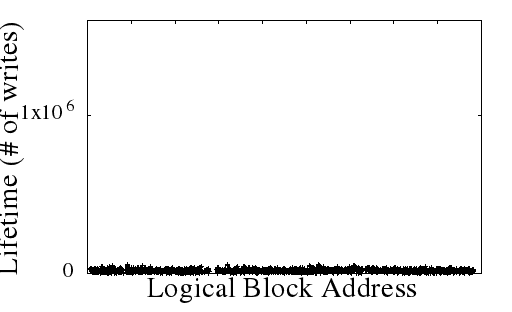
\includegraphics[scale=0.4]{figure/pcstream/type_1}} % data from 4/03031953 
	\hspace{10pt}
	\subfigure[Logging (manual)]{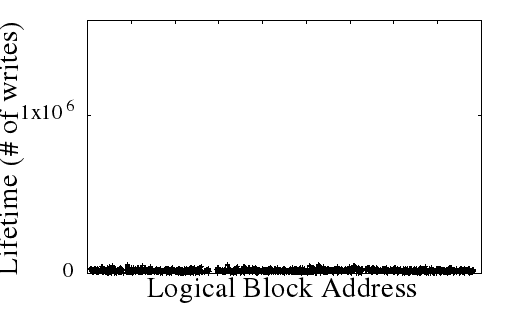
\includegraphics[scale=0.4]{figure/pcstream/pcID_2}}
	 \\
	\subfigure[Flushing (PC)] {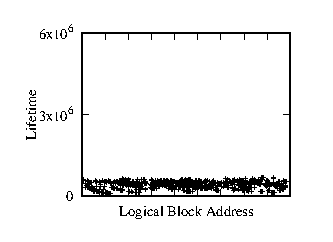
\includegraphics[scale=0.4]{figure/pcstream/type_3}}
	\hspace{10pt}
	\subfigure[Flushing (manual)]{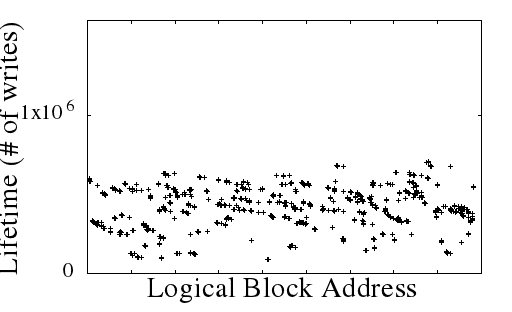
\includegraphics[scale=0.4]{figure/pcstream/pcID_3}}
\caption{Data lifetime distributions of different PCs.} 
\label{fig:types_and_PCs}
\end{figure}


In order to validate our hypothesis that PCs can be useful for predicting
lifetimes by distinguishing dominant I/O activities, we conducted experiments
using RocksDB, comparing the accuracy of identifying dominant I/O activities
using two different methods.  First, we manually identified dominant I/O
activities by inspecting the source code. Second, we automatically decided
dominant I/O activities by extracting PCs for write-related system functions.
Fig.~\ref{fig:types_and_PCs} illustrates two dominant I/O activities matched
between two methods.   As shown in Fig.~\ref{fig:types_and_PCs}(a)
and~\ref{fig:types_and_PCs}(b), the logging activity of RocksDB is correctly
identified by two methods.  Furthermore, from the logging-activity PC, we can
clearly observe that data written from the PC are short-lived. Similarly,
from Fig.~\ref{fig:types_and_PCs}(c) and~\ref{fig:types_and_PCs}(d), we observe
that data written from the flushing-activity PC behave in a different fashion.
For example, data from the flushing-activity PC remain valid a lot longer than
those from the logging-activity PC.

\section{Design of \textsf{PCStream}}
%We describe in detail the proposed automatic stream management technique, 
In this section, we describe in detail the proposed automatic stream management technique, %shane part
\textsf{\small PCStream}.  We first explain how we automatically extract PCs during
runtime and describe how multiple PCs are mapped to streams in an SSD.
In order to mitigate the side effect of a few outlier PCs with large lifetime variances, 
we introduce `substreams' based on a two-phase
stream assignment technique.
%{\it The PC extractor module}, which is implemented in the ... as part ... of a
%system call handler, computes a PC signature (i.e., a sum of program counter
%values) for each write-related system function. 추가 동작 설명..


Fig.~\ref{fig:architecture} shows an overall organization of \textsf{\small PCStream}.
\textit{The PC extractor module}, which is implemented in the Linux kernel as
part of a system call handler, 
computes a PC signature, which is used as a unique ID for each program context.  
We use the signature program counter~\cite{PC} as a PC signature 
by summing program counter values along the execution path to a write-related system function 
(e.g., {\tt write()}).  
With the PC signature, we can monitor the data lifetime of each write at the program context level. 
A PC signature value is stored
in an inode data structure of a file system (modified for \textsf{\small PCStream})
and is delivered to \textit{the lifetime analyzer module} which estimates
expected lifetimes of data belonging to a given PC in the block device level.
In order to efficiently detect the end of data lifetime in append-only
workloads, the lifetime analyzer also intercepts TRIM~\cite{TRIM} requests. %from a file system.  %shane part
Based on the lifetime information, \textit{the PC-to-stream
mapper module} clusters PCs with similar lifetimes and maps them together to
the same stream ID.  This mapping is required because 
the number of streams in an SSD is generally less than the number of PCs in host applications.

\subsection{Automatic PC computation}
As mentioned earlier, a PC is represented by a PC signature which is defined as
the sum of program counter values along the execution path of a function call that
%finally 
reaches a write-related system function. A function call involves
pushing the next program counter, which is used as a return address, to the
stack followed by pushing a frame pointer value.  In general, by using frame
pointer values, we are able to back-track the stack frames of the process and
selectively get return addresses for generating a PC signature.  For example,
Fig.~\ref{fig:getpc}(a) shows the abstracted execution path for flushing data
in RocksDB and Fig.~\ref{fig:getpc}(b) illustrates how a PC signature is obtained
by back-tracking the stack.  
Since a frame pointer value in the stack holds the address of the previous
%frame pointer, the PC extractor can easily obtain return addresses and
frame pointer, the PC extractor can obtain return addresses and
accumulate them to compute a PC signature. 
%(The return addresses are pushed
%before calling the \textsf{\small  write()}, \textsf{\small  BuildTable()} and \textsf{\small 
%WriteLevel0Table()} functions.)

\begin{figure}[t]
	\centering
	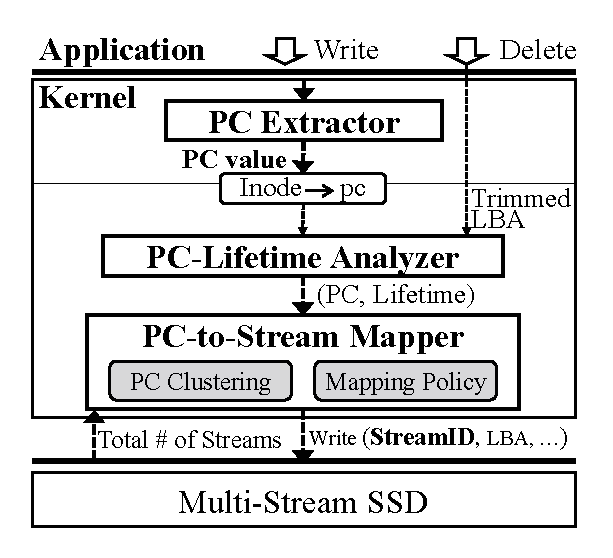
\includegraphics[width=0.6\linewidth]{figure/pcstream/architecture4}
	\caption{An overall architecture of \textsf{\small PCStream}.}
	\label{fig:architecture}
\end{figure}

%The PC extractor obtains and accumulates each
%return address, which is pushed before calling the \textsf{\small  write()}, \textsf{\small 
%BuildTable()} and \textsf{\small  WriteLevel0Table()} functions, by referring the frame
%pointer which holds the address of the previous frame pointer.

%Unfortunately, C/C++ compilers often optimize an output code so
%that it does not use a frame register if possible.  
The frame pointer-based approach for computing PC signatures, however, is not
always possible because modern C/C++ compilers often do not use the frame
pointer for improving the efficiency of register allocation.
One example is a
{\tt -fomit-frame-pointer} option of GCC~\cite{GCC}. 
%While it is effective in saving
%precious resources like CPU registers, this makes it difficult for us to
%back-track return addresses only. 
Although this option allows the frame pointer to be used as a general-purpose
register for high performance, it makes very difficult for us to back-track
return addresses along the call chains.  

\begin{figure}[t]
	\centering
	\subfigure[An abstracted execution path for flushing data.]{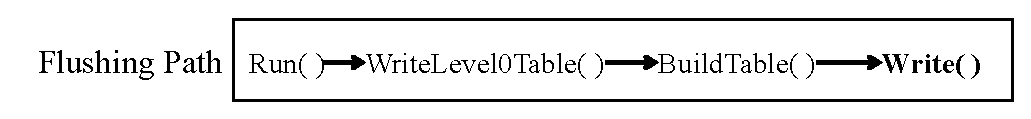
\includegraphics[scale=0.6]{figure/pcstream/getpc_1}}  
	\\
	\subfigure[with the frame pointer.]{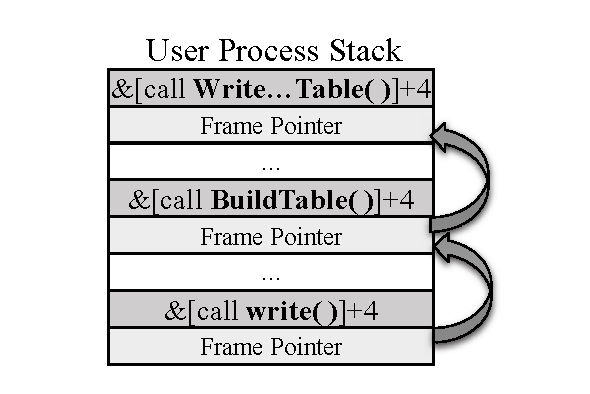
\includegraphics[scale=0.55]{figure/pcstream/getpc_2}}
	\hspace{10pt}
	\subfigure[without the frame pointer.]{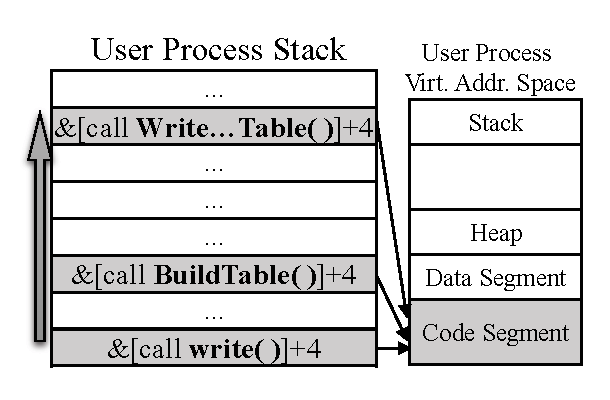
\includegraphics[scale=0.55]{figure/pcstream/getpc_3}}
	%\caption{An example execution path and its PC extraction methods.}
	\caption{An example execution path and its PC extraction.} %shane part
	\label{fig:getpc}
\end{figure}

In \textsf{\small PCStream}, we employ a simple but effective workaround 
for backtracking the call stack when the frame pointer is not used.
When a write system call is made, we scan every word in the stack and check
if it belongs to the process's code segment.  If the scanned stack word holds a
value within the address range of the code segment, we assume that it is a
return address.  Since scanning the full stack takes too long, we stop the
stack scanning procedure when a sufficient number of return address candidates
are found.  In the current version, we stop when 5 return address candidates
are found.  Although quite ad-hoc, a restricted scan is effective in
distinguishing different PCs because two different PCs
cannot follow the same execution path to write system functions.  
(If they do, they are the same PC.) In our evaluation
with a 3.4 GHz CPU machine, the performance overhead of the restricted scan was
almost negligible, taking only 300-400 $n$sec per write system call.

\subsection{PC lifetime prediction}

The prediction of PC lifetimes is rather complicated. 
The data lifetime of the append-only workload is defined 
from when a write request is issued until the TRIM command~\cite{TRIM} is issued to 
the corresponding address.
In order to measure the lifetime of data, the lifetime analyzer 
records the write time and PC value for each write request using its LBA.
Upon receiving the TRIM command, the lifetime analyzer can compute the 
lifetime of the corresponding data using the recorded information.
Note that, the
same PC may generate multiple data streams with different lifetimes.
We take the average lifetime as the PC's lifetime.

\subsection{Mapping PCs to SSD streams}

The last step in \textsf{\small PCStream} is to map
a group of PCs with similar lifetimes to an SSD stream.
This is because each SSD supports a limited number of stream IDs. For
example, SSDs used in \textsf{\small FStream}~\cite{FStream} and \textsf{\small AutoStream}~\cite{AutoStream}
support only 9 and 16 streams, respectively. To properly group multiple PCs,
the PC-to-stream mapper employs a simple 1-D clustering algorithm. 
In order to cluster PCs with similar lifetimes, the mapper calculates the 
lifetime difference between PCs.
Then, PCs with the smallest lifetime difference are clustered into the same PC group. 
The mapper repeats this clustering step until all the PCs are assigned to their PC groups.
For adapting to changing
workloads, reclustering operations should be regularly performed. Since the
number of PCs created by applications is not limited, the clustering algorithm
must be efficient enough to quickly handle many PCs. Our goal in this work is
to confirm the feasibility of using PCs, so we leave
those issues as our future work.

\subsection{Two-phase stream assignment}

For most PCs, their lifetime distributions tend to have small variances.  
However, we observed that a few outlier PCs which have large lifetime variations. 
For example, when multiple I/O contexts are covered by the same write system function, 
the corresponding PC may represent several I/O contexts whose data lifetimes are quite different.   
Such a case occurs %, for example, 
in the compaction module of RocksDB.
RocksDB maintains
several levels, L1, ..., L$n$, in the persistent storage, except for L0 (or a
memtable) stored in DRAM.  Once one level, say L2, becomes full, all the data
in L2 is compacted to a lower level, i.e., L3.  It involves moving data from L2
to L3, along with the deletion of the old data in L2.  In the
LSM tree~\cite{LSM}, a higher level is smaller than a lower level 
(i.e., the size of (L2) $<$ the size of (L3)). 
Thus, data stored in a higher level is invalidated more frequently than those kept
in lower levels, thereby having shorter lifetimes.

%Once the L1 becomes full,
%\textit{all} the data kept in the L1 are moved to the L2 by the compaction
%module.  The same operation is applied to the other levels (i.e., L3, ...,
%L$n-1$).  The compaction involves reading and writing data from a higher level
%(e.g., L1) to a lower level (e.g., L2).  The data in a higher level (e.g., L1)
%is then removed.  

%While the program context can be used as a useful indicator that determines the
%lifetime of data, we also observe that the same PC could generate data 
%with diverged lifetimes. One of the representative examples is the compaction
%module of RocksDB. RocksDB maintains several levels, L1, ..., L$n$, in the
%persistent storage, except for L0 (or a memtable) stored in DRAM.  Data flushed
%from the memtable are first written to the L1.  Once the L1 becomes full,
%\textit{all} the data kept in the L1 are moved to the L2 by the compaction
%module.  The same operation is applied to the other levels (i.e., L3, ...,
%L$n-1$).  The compaction involves reading and writing data from a higher level
%(e.g., L1) to a lower level (e.g., L2).  The data in a higher level (e.g., L1)
%is then removed.  In the LSM-tree, a higher level is smaller than a lower
%level. Thus, data stored in a higher level is invalidated sooner than data kept
%in lower levels, thereby having much shorter lifetimes.

Unfortunately, in the current RocksDB implementation, the compaction step is supported 
by the same execution path (i.e., the same PC) regardless of the level.
Therefore, the PC for the compaction activity cannot effectively separate data with 
short lifetimes from one with long lifetimes.
Fig.~\ref{fig:compaction}(a) shows 
the lifetime distribution collected from the compaction-activity PC.  
Since this distribution includes lifetimes of data written from all the levels, 
its variance is large.  
When we manually separate the single compaction step into several per-level compaction steps, 
as shown in Figs. 5(b) and 5(c), the lifetime distributions of per-level compaction steps 
show smaller variances.   
In particular, L2 and L3 show distinct lifetime distributions from that of L4.
Data from L2 and L3 are likely to have shorter lifetimes, while L4 has generally
long-lived data as shown in Fig. 5(d).

\begin{figure}[!t]
\centering
\subfigure[compaction: all levels]{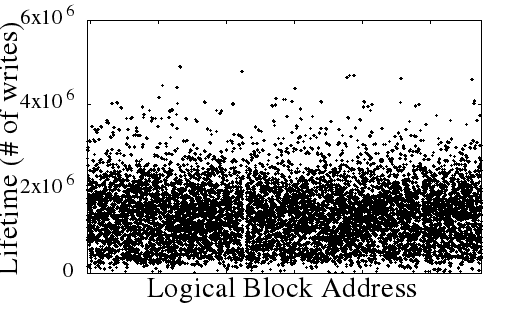
\includegraphics[scale=0.4]{figure/pcstream/pc_3}}
	\hspace{10pt}
\subfigure[compaction: L2]{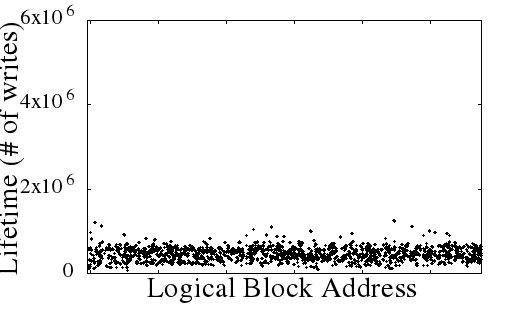
\includegraphics[scale=0.4]{figure/pcstream/type_4}}  % data from 4/03040047
\\
\subfigure[compaction: L3]{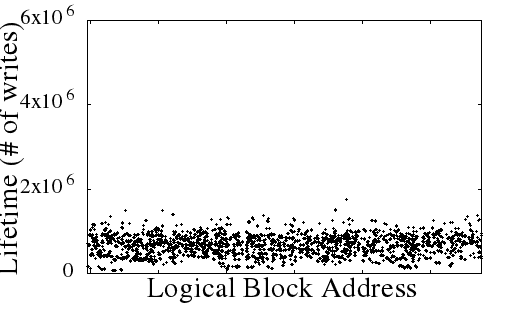
\includegraphics[scale=0.4]{figure/pcstream/type_5}}
	\hspace{10pt}
\subfigure[compaction: L4]{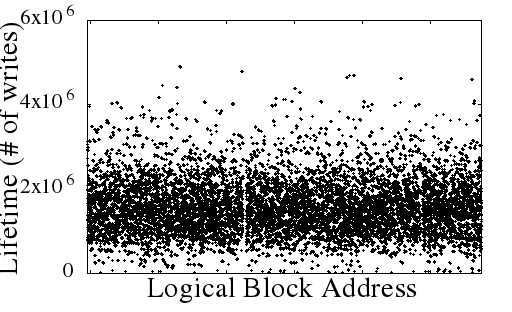
\includegraphics[scale=0.4]{figure/pcstream/type_6}}
%\caption{The lifetime distribution of the compaction activity.} 
\caption{Lifetime distributions of the compaction activity at different levels.} %shane part
\label{fig:compaction}
\end{figure}

Since it is difficult to separate data with different lifetimes within the same PC 
(as in the compaction-activity PC), we devised a two-phase method that decides SSD 
streams in two levels: the main stream ID in a host level and the substream ID in an SSD level.
Conceptually, long-lived data in the main stream are moved to its substream to 
separate from (future) short-lived data of the main stream.
Although moving data to the substream may increase WAF,
the overhead can be hidden if we restrict the substream move during GC only.
Since long-lived data (i.e., valid pages) in a victim block are moved to a free block during GC, 
they can be moved to the substream by changing the target block.
For instance, \textsf{\small PCStream} assigns the compaction-activity PC {\it pID} to a
main stream {\it sID} for the first phase.
To separate the long-lived data of {\it pID} (e.g., L4 data) 
from future short-lived data of {\it pID} (e.g., L1 data), 
valid pages of the {\it sID} are assigned to its substream for the second phase during GC.


\section{Experimental Results}

For our experiments, we have implemented \textsf{\small PCStream} in the Linux kernel
4.5.  For an objective evaluation, we compared \textsf{\small PCStream} with three
existing schemes: \textsf{\small Baseline}, \textsf{\small Manual}~\cite{MultiStream}, and
\textsf{\small AutoStream}~\cite{AutoStream}.  \textsf{\small Baseline} stands for a legacy
SSD that does not support a multi-stream feature. \textsf{\small Manual} is a RocksDB
implementation which is manually optimized for multi-streamed SSDs.
\textsf{\small AutoStream} is an LBA-based data separation technique which is
implemented at the device driver layer. To understand the impact of the
two-phase assignment, in addition, we compared \textsf{\small PCStream} with
\textsf{\small PCStream$^{*}$} which excluded the two-phase assignment feature.

For benchmarks, we have used three scenarios of \texttt{db\_bench} of RocksDB:
Update-Random (\texttt{UR}), Append-Random (\texttt{AR}), and Fill-Random
(\texttt{FR}) scenarios.  For key-value pairs already stored in the SSD,
\texttt{UR} updates values for random keys, creating many
read-modify-writes in the SSD.  \texttt{AR} is similar to \texttt{UR}, except
that it performs the update of values for growing keys. \texttt{FR} writes
key-value pairs to the SSD in a random key order.

\subsection{Experiments with an SSD emulator}

We carried out a set of experiments using an SSD emulator which is based on the
open flash development platform~\cite{AMF}.  
%The SSD emulator emulates the behaviors of an SSD using host DRAM in the kernel level. Thus, it not only allows us to easily add new features, but enables to analyze detailed internal activities of an SSD. 
In the SSD emulator, the internal workings of an SSD are simulated using the host's DRAM memory in the kernel level. 
For our evaluations, we extended the SSD emulator to support a multi-streamed feature %.
(up to 8 streams). %shane part
Furthermore, we enhanced the garbage collection module of the SSD firmware to support the two-phase stream management technique. 
%We assume that the SSD emulator supports up to 8 streams (as with Samsung PM963 which was used in our experiments). %shane part
%We enhanced the original emulator so that it supported a multi-streamed feature as well as the two-phase stream assignment.  The number of streams supported by the emulator was 8.  
The SSD emulator provided 12 GB capacity with 4 channels and 4 ways, and there were 8192 flash blocks, each of which was composed of 384 4-KB pages.  

\begin{figure*}[t]
	\centering
	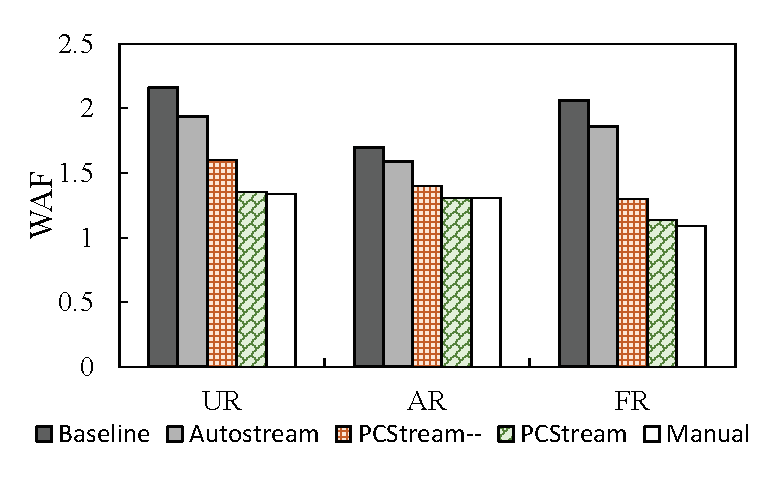
\includegraphics[scale=0.6]{figure/pcstream/result_emul}
	\caption{A comparison of WAF on the SSD emulator.}
	\label{fig:result_emul}
\end{figure*}


We compared WAF of the existing techniques with \textsf{\small PCStream} for the three
scenarios, and the result is shown in Fig.~\ref{fig:result_emul}.
\textsf{\small PCStream} was quite effective in reducing WAF, 
thus achieving an equivalent level of the WAF reduction as in \textsf{\small Manual}.  
For example, both \textsf{\small PCStream} and \textsf{\small Manual} reduced WAF by 38\% over \textsf{\small Baseline} for the \texttt{UR} case. 
%Compared with \textsf{\small AutoStream}, \textsf{\small PCStream} was more effective, reducing WAF more by 35\% on average.  
\textsf{\small PCStream} outperformed \textsf{\small AutoStream} by reducing WAF by 35\% on average.
Fig.~\ref{fig:result_emul} also indicates that the two-phase stream assignment technique is effective.  
\textsf{\small PCStream} outperformed \textsf{\small PCStream$^{*}$} by 12\% on average in the WAF reduction.
%As shown in Fig. 6, \textsf{\small PCStream$^*$} reduced WAF by up to 30\% over \textsf{\small AutoStream}.  
%The result shows that separating short-lived data (e.g., log and flush) from long-lived one (e.g., compaction) using PC was quite effective in reducing WAF.  Moreover, \textsf{\small PCStream} even showed similar WAF to \textsf{\small Manual}, reducing it by up to 38\% over \textsf{\small AutoStream}.  
This additional gain of \textsf{\small PCStream} over \textsf{\small PCStream$^{*}$} came from isolating long- and short-lived data in separate blocks 
%through the two-phase assignment at the SSD even if they belonged to the same compaction PC.
%by moving the long-lived data of the compaction-activity PC to substreams during GC at the SSD.
by moving the long-lived data to substreams during GC at the SSD.


In order to better understand how \textsf{\small PCStream} achieved a high reduction in WAF, 
we measured per-stream lifetime distributions under each technique for the \texttt{UR} scenario.
Fig.~\ref{fig:stream_lifetime} shows a box plot of data lifetimes from the 25th percentile to the 75th percentile.
%In order to analyze the improvement made by \textsf{\small PCStream}, 
%we measured the data lifetime of each stream for the {\tt UR} scenario.
%Fig. 7 shows average, 75p, and 25p of data liftime for each stream.

\begin{figure*}[t]
	\centering
	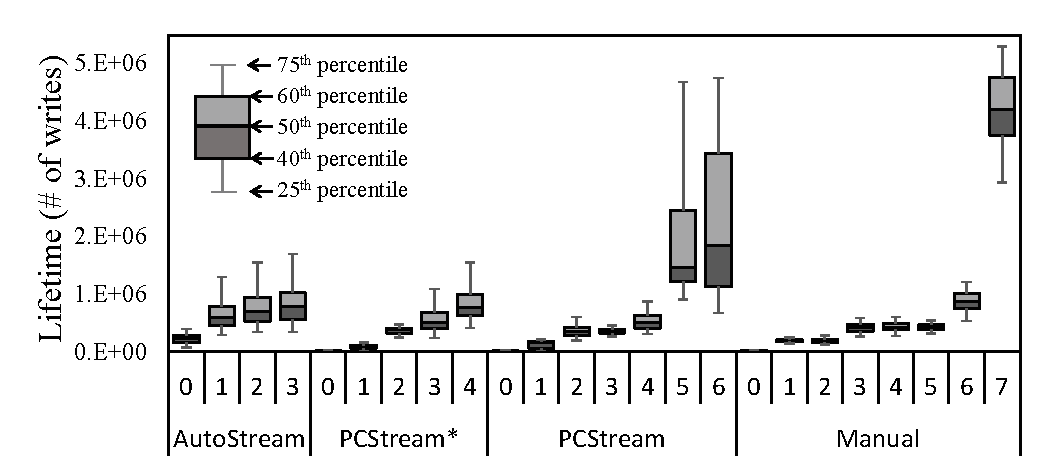
\includegraphics[scale=0.6]{figure/pcstream/stream_lifetime}
	\caption{A comparison of per-stream lifetime distributions.}
	\label{fig:stream_lifetime}
\end{figure*}



As shown in Fig.~\ref{fig:stream_lifetime}, 
streams in \textsf{\small PCStream} are divided into two groups, 
$G1$ = $\{$0, 1, 2, 3, 4$\}$ and $G2$ = $\{$5, 6$\}$, 
where $G1$ includes streams with short lifetimes and small variances %(i.e., streams 0, 1, 2, 3, and 4) 
and $G2$ includes streams with large lifetimes and large variances.  %(i.e., streams 5 and 6).  
%By preventing $G1$ and $G2$ from mixing in the same block, \textsf{\small PCStream} can reduce the GC overhead.  
Since the GC copy cost is affected by how data in $G1$ and $G2$ are mixed into the same block, 
\textsf{\small PCStream} can significantly reduce the GC overhead 
by avoiding such data mixtures in the same block by separating $G1$ and $G2$ into different streams. 
On the other hand, in \textsf{\small AutoStream}, 
three streams (i.e., streams 1, 2, and 3) show similar lifetime distributions with large variances 
without a distinct data separation pattern.
%Unlike \textsf{\small PCStream} and \textsf{\small Manual}, \textsf{\small AutoStream} does not show that 
%their streams are divided based on data lifetimes.  
%Such stream allocation is not effective in reducing the GC copy cost. 
%, thus not effectively taking full advantage of streams.
%data lifetimes of stream 0 to 5 in \textsf{\small Manual} are gathered in a narrow range so data lifetime in the same is quite similar.
%However, data lifetime of streams in \textsf{\small AutoStream} shows relatively large difference
%\textsf{\small AutoStream} does not notice when long-lived data is written to the hot stream.
%On the other hand, \textsf{\small PCStream$^*$} can identify short-lived data from 
%several dominant I/O activities as mentioned in section 2, for example, stream 0 and 1 in the Fig.~\ref{fig:stream_lifetime}.
%\textsf{\small PCStream} can further separate long-lived data of several streams (e.g., stream 3 and 4)
%by moving their data to substreams (e.g., stream 5 and 6, respectively). 
In Fig.~\ref{fig:stream_lifetime}, we can also observe the effect of substreams.  
Streams 3 and 4 of \textsf{\small PCStream$^{*}$}, 
which have large variances in lifetimes, are split into two substreams 5 and 6 in \textsf{\small PCStream}.
This split reduces variances of streams 3 and 4, thus reducing the GC copy cost.  %improving WAF. 

\subsection{Experiments with a real-world SSD}

In order to evaluate the effect of \textsf{\small PCStream} in a real SSD,  
%In order to confirm the feasibility of \textsf{\small PCStream}, 
we have
conducted experiments using Samsung's PM963 480GB SSD that supports 8 streams.
Since it was impossible to implement the two-phase stream assignment in the
commercial SSD firmware, we evaluated \textsf{\small PCStream$^*$} only.  To warm up the
SSD before running benchmarks, we filled up 90\% of the SSD capacity with valid
data.

\begin{figure*}[t]
	\centering
	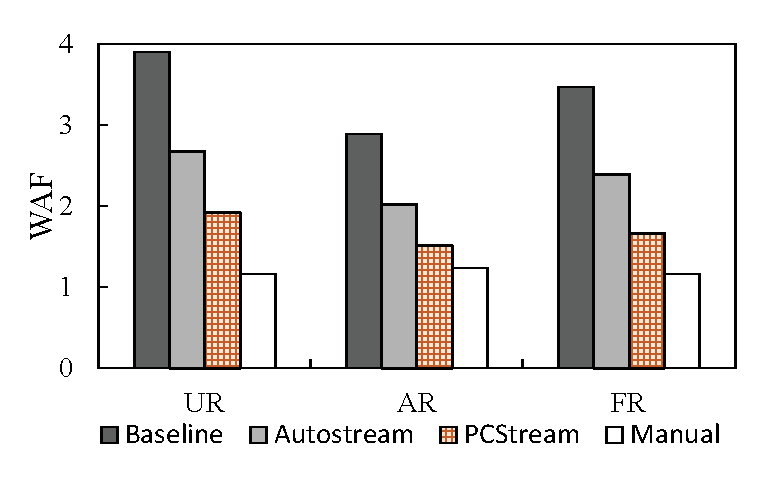
\includegraphics[scale=0.6]{figure/pcstream/result_ssd}
	\caption{A comparison of WAF on Samsung PM963 SSD.}
	\label{fig:result_ssd}
\end{figure*}


As illustrated in Fig.~\ref{fig:result_ssd}, \textsf{\small PCStream$^*$} reduced WAF by
28\% over \textsf{\small AutoStream} on average.  
%There were large WAF gaps between \textsf{\small PCStream$^{*}$} and the manually optimized case.  If the substream was properly supported during GC, we believe that \textsf{\small PCStream} could show similar WAF values as \textsf{\small Manual}.  
Note that although \textsf{\small PCStream$^*$} still outperformed \textsf{\small AutoStream} in PM963, 
but a performance gap was smaller over that
in the emulated SSD environment.  It was difficult to pinpoint why
\textsf{\small AutoStream} worked better in PM963 over in the emulated SSD, but we
suspect that some internal features of PM963 (such as a large block size or some implementation details of streams) %might be related. 
might have affected the performance of \textsf{\small AutoStream}.


\section{Conclusions}

We have presented a new stream management technique, \textsf{\small PCStream}, for multi-streamed SSDs.  
Unlike existing stream management techniques, \textsf{\small PCStream} fully automates 
the process of mapping data to a stream based on PCs, 
which work well for append-only workloads as well as update workloads.  
By exploiting an observation that most PCs are distinguishable from each other 
in their lifetime characteristics, \textsf{\small PCStream} allocates each PC to a different stream.  
When a PC has a large variance in their lifetimes, \textsf{\small PCStream} refines its stream allocation 
during garbage collection and moves the long-lived data of the current stream to its substream.  
%Our experimental results show that \textsf{\small PCStream} can reduce WAF by up to 38\% over the existing
Our experimental results show that \textsf{\small PCStream} can reduce the average WAF by 35\% over the existing %shane part
automatic technique.

The current version of \textsf{\small PCStream} can be extended in several directions.  
For example, we plan to optimize the PC clustering method so that
multiple PCs can be better clustered when the number of PCs significantly
outnumbers the number of streams.  
%For example, \textsf{\small PCStream} should be improved in its PC clustering method 
%so that it can work effectively even when there are more PCs than the number of streams.  
%We also plan to evaluate \textsf{\small PCStream} (not \textsf{\small PCStream}$^{--}$) on real SSDs 
%by implementing the two-phase stream assignment algorithm inside an FTL.
